%% The following is a directive for TeXShop to indicate the main file
%%!TEX root = diss.tex

%=======================================
\chapter{Introduction}
\label{ch:Introduction}
%=======================================

Why do we study random walks? Apart from being an interesting mathematical object that leads to a lot of interesting mathematics, they have some real world applications. A lot of processes can be modeled via random walks - from stock market objects to proteins and polymers. There is a rich theory of continuous and discrete random walks. Specifically in random walk enumeration we attempt to find out things about the numbers of walks of some length and of certain type with certain geometrical constraints. The topic often leads to the use of generating functions as a powerful tool in the analysis. In the end we gain insight into what makes certain random walk models "easy" and others more difficult. In this thesis we look at the enumeration for constrained random walks with interactions in order to gain insight into the deeper workings of random walk enumeration problems.
%=======================================
\section{Recent History}
%=======================================

With the terminology from autoref{ch:Preliminaries} in place we are ready to discuss some of the recent history of random walk enumeration. In the most basic case random walks starting at the origin on $d$ dimensions have no restrictions $\mc{D}$ is the whole space and there are no interactions. We can enumerate these walks easily by writing the full generating function
\begin{align}
\begin{split}
	Q(\row xd;t) &= \frac{1}{1-tS(\row xd)} \\
			&= 1 + tS(\row xd) + t^2 S(\row xd)^2 + \cdots\,.
\end{split}
\end{align}
This works since we can use each individual steps and every walk is uniquely represented by a sequence of steps from $\mc{S}$. This works for arbitrary initial conditions too since we can start the walks at any point and evolve them. The coefficients of each power of $t$ are Laurent polynomials in the variables $\row xd$. If we have the generating function for a random walk model we have a lot of information at our hands. Replacing $x_k$ with $0$ for each $k$ gives us the generating function for walks returning to the origing. Similarly taking higher derivatives and evaluating at zero allows us to find the number of walks ending at specific points. If we set all the $x_k = 1$ inf $Q$ we obtain the length generating function for the random walks in the plane. There are numerous questions we can ask about each of those characteristics of the model.

The nest step up is to deal with half-spaces - here $\mc{D}$ is the region where one of the $x_k \ge 0$. These cases are not as simple to solve but they are doable. Check \cite{gessel1980factorization}, \cite{bousquet2000linear}, \cite{duchon2000enumeration} and \cite{banderier2002basic} for work on the one-dimensional case that can be extended to general $d$. The generating functions we can obtain are algebraic. Naturally we are led to consider cases where $\mc{D}$ is an intersection of half-spaces. Even for $d=2$ the problem has generated a rich theory of quadrant (or quarter-plane) walks. We obtain functional equations for the function $Q$ that are not easy to solve in general - often the generating functions here are not even D-finite although there are D-finite examples. The main object of study in these cases has been a group $G$ of bi-rational transformations preserving the polynomial $K = 1- tS$ called the kernel of the model. 

When $G$ is finite (in the 23 non-equivalent cases) we obtain a D-finite generating function (full?) as can be seen the classifications \cite{mishna2009classifying},\cite{bousquet2010walks} and \cite{bousquet2005walks}, \cite{bostan2010complete} for specific cases. The main tool in the study of the finite group cases has been the algebraic kernel method in which we sum different functional equations produced by group actions by elements of $G$ in order to cancel the majority of the terms in the functional equation. See \cite{kauers2014walks} for treatment of models with repeated steps with finite groups.

 There are 56 non-equivalent cases of quarter-plane walks with an infinite group. For 51 of them both the full generating function \cite{kurkova2011explicit} and the length generating function for walks returning to the origin are not D-finite \cite{bostan2014non}. The remaining 5 cases have been dealt with in \cite{melczer2014singularity} and \cite{melczer2014variants}. The main tool used to tackle these 5 cases is the iterated kernel method in which we use the roots of the kernel $K$ to show the generating function is not D-finite.

Naturally we are led to invesitigating higher-dimensional variants of this problem. See \cite{gessel1992random} and \cite{grabiner1993random} for when $\mc{D}$ is a Weyl chamber. In three dimensions we have the recent partial classification \cite{bostan2014three} of random walk models with up to six steps where the authors extend the algebraic kernel method to handle the majority of finite group cases encountered.

Another generalization is to consider walks with interactions and/or self-avoiding walks (or SAWs). These two types of generalizations have important applications in physics because they can be used to model polymers, proteins and other chains. For some research on SAWs with various interactions see \cite{van2004multiple},\cite{brak2009self}, \cite{wong2014confining} \cite{chan2012monte}, \cite{bacher2011weakly}, \cite{bedini2014lattice} and \cite{dagrosa2015writhe}. The topic of SAWs doesn't lend itself as nicely to using generating functions like the ones considered so far so as a simpler first step we can consider regular random walks with interactions. See \cite{niederhausen2005random} and \cite{niederhausen2005note} for walks with interactions in an octact. See \cite{brak2005directed}, \cite{owczarek2012enumeration}, and \cite{tabbara2014exact} for walks with interactions in the plane.

A long-standing dream goal in random walk enumeration research is the automatization of the process of determining characteristics of the models and similar problems. There has been some progress in this direction. See for example \cite{gessel1990symmetric} and \cite{chyzak2005effective} for details on symmetric functions, \cite{mishna2005holonomic} for a holonomic approach to combinatorics, \cite{bostan2009automatic} for automatic classification of lattice walks, and finally \cite{kauers2011computational} for some of the computational challenges involved in automation.

A related subject of study is the asymptotics of random walks where some automation can be performed. For examples of the theory see \cite{johnson2013towards}, \cite{melczer2014asymptotic} and \cite{melczer2014enumerating}. A lot of the works mentioned so far have also discussed asymptotics.

%=======================================
\section{Thesis Objectives}
%=======================================

This thesis grew out of work on regular quadrant random walks with interactions with the axes. The derivation of the functional equation in the non-interacting case is a simple inclusion-exclusion process but doing the same for the interacting case is somewhat more involved. It is possible to further simplify the equation via coefficient extraction and back-substitution. It works out beautifully to give us a much more compact functional equation. However, the process is quite painstaking even for three dimensions, let alone for higher-dimensions, although it is possible. 

The mathematicians who study random walk enumeration have as a goal to classify random walks according to various characteristics like step set, dimension, group size associated to the kernel, and perhaps most importantly - D-finitenes. They also dream of being able to make the process automatic whenever it is possible. In this thesis we aim to further the study of random walk models towards this goal of automatization. We might as well be as optimistic as possible and suppose that a general algorithm exists that takes an arbitrary random walk model - in arbitrarily many dimensions, with arbitrary finite step sets and with arbitrary constraints, and outputs various data about the model - functional equation for the generating function, a solution and information about the model's D-finiteness. It is only logical that if such an algorithm were to exist it would not have difficulty with the particulars of the random walk model. While this kind of algorithm may be too strong to envision (it may be the case that there are atrocious random walk models which we cannot solve), the idea of the existence of such an algorithm has been a strong motivator in our pursuit of generalization. This thesis succeeds in demonstrating that the first task is achievable. For a vast assortment of random walk models we can almost-automatically write down a functional equation for its generating function counting length, position and interactions of the random walks. The equation looks like
\begin{align}
	(1- t\Gamma S) Q = q
\end{align}
where $\Gamma$ is an operator on the variables of $Q$, $S$ is the Laurent step polynomial (keeping inventory of the steps in polynomial form) and $q$ is some Laurent polynomial initial condition. The operator idea is powerful and we'll use it as much as we can in this thesis. A secondary achievement is the furthering of the theory of the orbit summation method which along with the obstinate kernel method combine in a nicer theory of operators consisting of group actions. However time and space have not been sufficient to go too far in these lines. Near the end we present some solutions and partial solutions to random walk problems in two dimensions with interactions. 

%=======================================
\section{Layout of Thesis}
%=======================================

In the first few chapters we go through motivating examples which will serve as a springboard into further generalizations. First we'll start off with one-dimensional random walks with and without interactions in \autoref{ch:1DExample}. Then we'll quickly move on to two-dimensional random walks in \autoref{ch:2DWalks}. On the way we'll develop some of the basic operator theory involved in the random walk models. In Chapter 4 we'll make a detour to random walks on a honeycomb lattice - a problem that will show some of the group-theoretic and operator tools. In Chapter 5 we'll tackle the $d$-dimensional random walk model functional equations using operators. In chapter 6 we'll finally go through operators in a much generality as we can, deriving all sorts of properties for them along the way. In chapter 7 we'll discuss generalizations of the random walk models and we'll push the operator notation as far as we can to see what kind of problem we can hope to tackle with the theory.

In Chapter 8 we'll become more practical and deal with group-theoretic operators relevant to both two-dimensional and higher-dimensional random walk models. In Chapter 9 we extend the persistent kernel method as much as we can for the two-dimensional interacting walks. Then in Chapter 10 we attempt to solve as many highly-symmetrical two-dimensional interacting models as we can via the vanishing kernel method. In Chapter 11 we work on some models with higher group orders.

%========================
\section{Notation and Conventions}
%========================

%========================
\subsection{Formal Series}
%========================
We will work in the setting of formal power series and Laurent series. Issues with convergence will not be addressed in much detail. If we are given a ring $R$ we may construct several formal objects with a commutative indeterminate $x$ with coefficients in $R$.
\begin{itemize}
\item $R[x]$: Ring of polynomials with monomials $x^k$ for integers $k\ge 0$.
\item $R[x,1/x]$: Ring of Laurent polynomials with monomials $x^k$ for integers $k$.
\item $R[[x]]$: Ring of formal power series with monomials $x^k$ for integers $k \ge 0$.
\item $R((x))$: Field of formal Laurent series with monomials $x^k$ for integers $k$.
\end{itemize}
We can also define their multivariate analogues like $\Rpring{x}{n}$, $\Rlring{x}{n}$ and their series counterparts $\Rpsring{x}{n}$ and $\Rlsring{x}{n}$. For a thorough treatment of the subject please see \cite{monforte2013formal}. When we work with a combination of objects coming from different rings/fields over the indeterminate $x$ we'll consider all objects as part of the most general ring/field at the time. If in doubt, we'll always work in the field of formal Laurent series. Given a sequence $(w_n)$ we may consider its generating function $W(x)$ given by $\sum_{n} w_n x^n$ which lives appropriately in one of the rings over $x$. The multivariate case for a multi-index sequence $(w_{n_1,\ldots,n_m})$ is defined analogously as
\begin{align}
	W(x_1,\ldots,x_d) = \sum_{n_1,\ldots,n_m} w_{n_1,\ldots,n_m} x_1^{n_1}\ldots x_m^{n_m}
\end{align}
whenever this series is a formal Laurent series. When we solve enumeration problems via generating functions we often need to extract particular coefficients from the formal polynomial/series. In the one-variable case we have the coefficient extraction operators on formal series
\begin{align}
	[x^n] W(x) = w_n\,.
\end{align}
The multivariate case is handled analogously with the caveat that whenever the number of variables extracted is less than the number of variables present we extract by treating these remaining variables as parameters. For a more detailed discussion please consult \cite{goulden2004comb}. When we deal random walk generating functions we often work with functional equations. In the broadest sense in this thesis we'll discuss functional equations which may involve a function $F$, the function evaluated at various arguments and various coefficient extractions of $F$. This will be done via operators so in the end we'll have a functional equation involving $F$ and operators. We'll write the identity operator as 1.
%========================
\subsection{Random Walk Models}
%========================
In this work we'll investigate random walk models on the $n$-dimensional lattice $\ze^n$. A specific model $\mc{M}$ will consist of several ingredients
\begin{itemize}
\item $\mc{S}$ : a finite set of steps that we can take from a point in $\ze^n$ to another point in $\ze^n$. In general this step set may differ from point to point (\eg a honeycomb lattice embedded in $\ze^2$). The steps themselves will be written as vectors $s = (s_1,\ldots, s_n)$. For example $\mc{S}$ could be a set of small steps defined by coordinates among $\{-1,0,1\}$. Another example is when we have more than one step of a given kind. 
\item $\mc{D}$ : a domain for the random walks. This is the region in $\ze^n$ where the random walks will live. The easiest cases involve the whole space or a half-space. Starting with quarter-plane regions the analysis becomes rather complicated. One can further constrain the walks to live on semi-infinite strips.
\item $\mc{D}_0$ : an interaction domain for the random walks. This is a sub-region in $\mc{D}$ and we'll want to count how many times random walks interact with it by stepping on coordinates that are part of it. We may count different points from $\mc{D}_0$ in different ways. This less-studied paradigm may involve marking visits to the origin, axes in two dimensions, various higher-dimensional hyperplanes, a cone, infinite strip, the sides of a box and so on.
\item $\mc Q$ : a set of random walks acting as an initial condition from which all other random walks evolve. This could be as trivial as starting with the empty walk ending at the origin to a set of infinitely many walks with some pattern.
\end{itemize}

\begin{figure}[H]
    \centering
    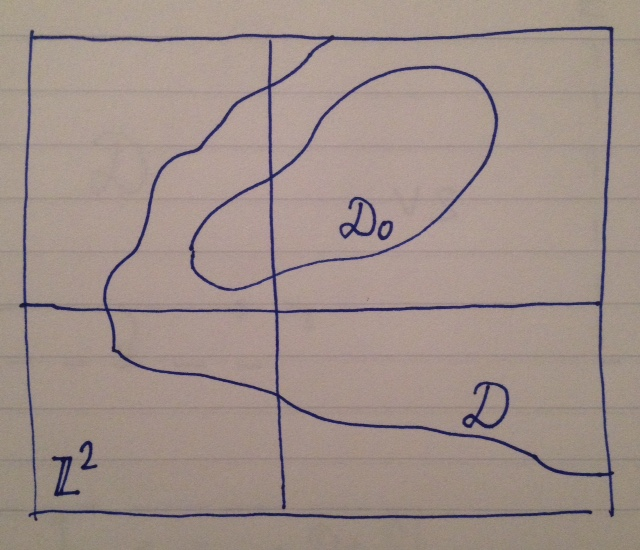
\includegraphics[scale = 0.5]{image1}
    \caption{The regions}
    \label{fig:fig1}
\end{figure}

It is natural to consider the generating function that will keep track of all the information characterizing the random walks in the model. For each random walk $w$ its length $|w|$ will be the total number of steps that it was taken and we'll keep track of it via a parameter $t$. We'll keep track of its endpoint coordinates in $\ze^n$ by the indeterminates $x_1,\ldots,x_n$ and its interactions with $\mc{D}_0$ via marking parameters $a_m$ where $m$ is some specific subscript index. The marking is highly dependent on the geometry of $\mc{D}_0$ and the way we want to count interactions. If the end coordinates of the random walk are $(m_1,\ldots,m_n)$ and if the marking monomial (a product of $a_m$'s) is $a(w)$ we can write the generating  function for the random walk model as
\begin{align}
	Q(x_1,\ldots,x_n;t) = \sum_{w \in \mc{M}} a(w) x_1^{m_1}\ldots x_n^{m_n} t^{|w|}\,.
\end{align}
Other important objects are the step polynomial (or characteristic polynomial) $S(x_1,\ldots,x_n)$ defined by
\begin{align}
	S(x_1,\ldots,x_n) = \sum_{s \in \mc{S}} x_1^{s_1}\ldots x_n^{s_n}
\end{align}
and the starting polynomial
\begin{align}
	q(x_1,\ldots,x_n;t) = \sum_{w \in \mc{Q}}  a(w) x_1^{m_1}\ldots x_n^{m_n} t^{|w|}\,.
\end{align}
Usually we see $S$ a Laurent polynomial of degree (or valuation) 1 in each variable and we have $q = 1$. Note that in all of these quantities the variables $a_m$ have been supressed from the notation. We can include those too whenever necessary especially if there are only finitely many of them. Furthermore it'll be useful to use the quantities $b = a - 1$ and $c = b/a = 1- \ol{a}$.
\begin{example} To illustrate the notation we'll investigate a random walk model on the plane. We'll look at random walks starting at the origin, restricted to the quarter plane, and which have only small diagonal steps. We'll count their interactions with the axes. In our terminology we have a random walk model $\mc{M}$ with $\mc{S}$ given by
\begin{align}
	\mc{S} = \{(-1,-1),(1,-1),(-1,1),(1,1)\}\,.
\end{align}
\begin{figure}[H]
    \centering
\[
	\modelgraphB 10100101
\]
    \caption{The model $\{$NW, NE, SW, SE$\}$}
\end{figure}
The region $\mc{D}$ consists of all points in $\ze^2$ with non-negative coordinates. Next $\mc{D}_0$ is composed of the two non-negative axes with overlap at the origin - we'll count visits to the origin as visits to each axis. Finally $\mc{Q}$ consists of the empty walk. In the language of generating functions we have $q = 1$ and
\begin{align}
	S &= S(x_1,x_2)  = x_1+\ol{x}_1+x_2+\ol{x}_2 = (x_1+\ol{x}_1)(x_2 + \ol{x}_2)\,.
\end{align}
We have a choice in naming the variables counting the interactions so we'll go with their defining quality (as this proves notationally simpler later on) - we mark the locations where one coordinate is zero. That is mark walks ending on $x_k = 0$ by incrementing the power of $a_k$ in the generating function. In this model the only first step we can take is $(1,1)$ which contributes a monomial $x_1x_2t$. From here on we can build on the single random walk of size one by taking a step in any of the four directions. This action lead to the following monomials.
ZZPICTUREZZ
\begin{itemize}
	\item $(1,1)$: monomial $x_1^2x_2^2 t^2$ since there are no interactions.
	\item $(1,\um1)$: monomial  $a_2x_1^2t^2$ since the walk lands on the $x_1$-axis with coordinate $x_2 = 0$.
	\item $(\um 1,1)$: monomial  $a_1x_2^2 t^2$ since the walk lands on the $x_2$-axis with coordinate $x_1 = 0$.
	\item $(\um1,\um1)$: monomial  $a_1a_2 t^2$ since the walk lands on the origin which is on both axes.
\end{itemize}
Since we've seen all the random walks of size at most 2 we see that the generating function $Q = Q(x_1,x_2;t)$ starts as
\begin{align}
\begin{split}
	Q  &=  1 + x_1x_2 t + (a_1a_2 + a_1x_2+a_2x_1 +x_1x_2)t^2 + \cdots\\
	& = 1 + x_1x_2 t+ (a_1+x_1)(a_2+x_2)t^2 + \cdots\,.
\end{split}
\end{align}
The fact that the first few coefficients factor in this case may be unexpected but it is due to the factoring of $S(x_1,x_2)$ itself. We'll see a more general result later.
\end{example}
%========================
\subsection{Thesis Notation}
%========================
In the interest of generalizing the problem-solving strategies involved in random walk enumeration we will need powerful notation to handle all the intricacies of the problem. In fact it is the notation itself that paved the way towards generalization because it is suggestive and points towards the deeper connections between the generating functions and quantities involved. With this thesis we aim to make this kind of notation more common in higher-dimensional random walk analysis. Typically in multivariate setting we see multi-index notation where a bolded, vectorial or even supressed notation denotes the collection of variables involved. We would use this notation as well but it is insufficient when working with restricted geometries for $\mc{D}$ and $\mc{D}_0$.
\begin{definition} Let $\oo := (0,\ldots,0)$ and $\pm \one := (\pm 1,\ldots, \pm 1)$ where we have as many terms in these sequences as needed in the specific context and let $[n] = \{1,\ldots, n\}$
\end{definition}
\begin{definition} For sequences $I = (i_1,\ldots, i_m)$ and $J = (j_1,\ldots, j_m)$ and a symbol $x$ we denote the monomial
\begin{align}
	x_I^J = x_{i_1}^{j_1}\cdots x_{i_m}^{j_m}.
\end{align}
with the special cases
\begin{align}
	x_I^{\one} = x_I, \quad x_I^{\um\one} = \frac{1}{x_I} = \ol{x}_I\,.
\end{align}
\end{definition}
\begin{definition} For sequences $I,J$ as before and indeterminate $x$ we denote the coefficient extraction 
\begin{align}
	[x_I^J] F= [x_{i_1}^{j_1}\cdots x_{i_m}^{j_m}]F = F_I^J
\end{align}
with special cases:
\begin{itemize}
	\item $F_I^{J} = F$ if $I$ is empty.
	\item $F_I^J = F_J$ if $I$ is the full set of variables ordered unambiguously.
\end{itemize}
We'll primarily be using this notation for extractions w.r.t. the $x$ variables in the generating functions but sometimes we'll be using such a coefficient extraction w.r.t. to other variables, most commonly $t$. We'll never mix such extractions with this notation.
\end{definition}
\begin{example}Here's an illustrative example of the notation. If $Q(x_1,x_2;t)$ is given as in the previous example we have
\begin{align}
	Q_1^0 = [x_1^0]Q(x_1,x_2) = Q(0,x_2) &= 1 + a_1(x_2+a_2)t^2+\cdots\,,\\
	\Qf{0,0} = Q_{0,0} = Q(0,0) &= 1 + a_1a_2 t^2+\cdots\,.
\end{align}
Furthermore we may write
\begin{align}
	S_1^{\um 1} &= [\ol{x}_1](x_1+\ol{x}_1)(x_2+\ol{x}_2) = x_2+\ol{x}_2
\end{align}
and $\Sf{\pm 1,\pm1}  = 1$.
\end{example}

\endinput

